% title page
\frame{
   \begin{center}
    \huge{子どもIT未来塾}\\

    \vspace{34pt}
	   {\huge 第5回}\\
	   {\huge Raspberry Piをリモコンにしてみよう}\\
    \vspace{24pt}
    \large{奥山 祐市}
    \vspace{10pt}
    \large{\the\year 年 8月19日}
  \end{center}
}

\begin{frame}[fragile]
    \frametitle{教材のアップデートをしよう}
    \begin{center}
        \begin{columns}
            \begin{column}{0.48\textwidth}
                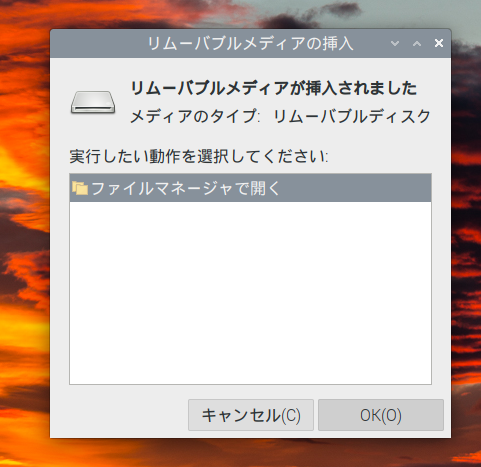
\includegraphics[width=\textwidth]{images/slide/insert_removal_media.png}
            \end{column}
            \begin{column}{0.48\textwidth}
                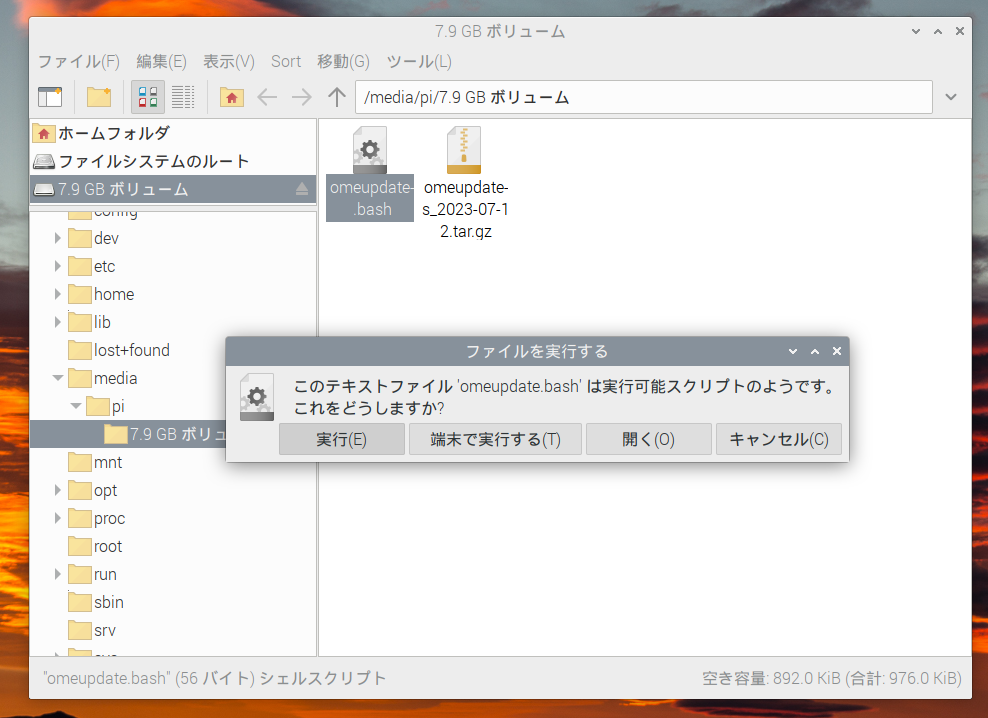
\includegraphics[width=\textwidth]{images/slide/exe_volume.png}
            \end{column}
        \end{columns}
        {USBメモリをラズパイにさして、教材をアップデートするプログラムを実行しよう}
    \end{center}
\end{frame}

\begin{frame}[fragile]
    \frametitle{目次}
    \begin{enumerate}
        \item センサーについて知ろう
        \item FaBoのセンサーを使ってみよう
        \item 赤外線について知ろう
        \item 赤外線を送信・受信してみよう
        \item 赤外線を使って家電を動かしてみよう
        \item 演習
    \end{enumerate}
\end{frame}
